\documentclass{beamer}

%------------------------------------
%------------Libraries---------------
%------------------------------------

\usepackage[utf8]{inputenc}
\usepackage{xpatch}
\usepackage{ragged2e}
\usepackage{xcolor}
\usepackage{url, hyperref}

\usepackage{amsmath, amsthm, amssymb, amsfonts, mathtools}
\usepackage{subfig}
\usepackage{booktabs}

\usepackage{tikz}
\usetikzlibrary{positioning, arrows.meta, shapes.geometric}

\usepackage{csquotes}
\usepackage[style=abnt]{biblatex}
\addbibresource{biblio.bib}

%------------------------------------
%----------Configurations------------
%------------------------------------

\usetheme{Madrid}
\usecolortheme{default}
\useinnertheme{circles}

\definecolor{FirstColor}{rgb}{0.0157, 0.2392, 0.4902}
\definecolor{SecondColor}{rgb}{0.0157, 0.5490, 0.8000}

\setbeamertemplate{itemize items}[triangle]

\setbeamercolor*{palette primary}{bg=FirstColor, fg=white}
\setbeamercolor*{palette secondary}{bg=SecondColor, fg=white}
\setbeamercolor*{palette tertiary}{bg=white, fg=FirstColor}
\setbeamercolor*{palette quaternary}{bg=FirstColor, fg=white}
\setbeamercolor{structure}{fg=FirstColor}
\setbeamercolor{section title}{fg=white}

\hypersetup{colorlinks=true, citecolor=blue, urlcolor=cyan, linkcolor=blue}

\apptocmd{\frame}{}{\justifying}{}

\AtBeginSection[]{
    \begin{frame}[plain,noframenumbering]
    \vfill
    \centering
    
\begin{tikzpicture}
        \node[
            fill=FirstColor,
            rounded corners=6pt,
            minimum width=0.85\paperwidth,
            minimum height=1.2cm,
            inner sep=0pt,
            text=white
        ]
        {%
            {\setbeamercolor{structure}{fg=white}
            \large\bfseries\secname}
        };
    \end{tikzpicture}
    \vfill
    \end{frame}
}

%---------------------------------------------------
%------------------Itemize--------------------------
%---------------------------------------------------

\makeatletter
\newcommand{\my@beamer@setsep}{%
\ifnum\@itemdepth=1\relax
     \setlength\itemsep{\my@beamer@itemsepi}%
   \else
     \ifnum\@itemdepth=2\relax
       \setlength\itemsep{\my@beamer@itemsepii}%
     \else
       \ifnum\@itemdepth=3\relax
         \setlength\itemsep{\my@beamer@itemsepiii}%
   \fi\fi\fi}
\newlength{\my@beamer@itemsepi}\setlength{\my@beamer@itemsepi}{3ex}
\newlength{\my@beamer@itemsepii}\setlength{\my@beamer@itemsepii}{1.5ex}
\newlength{\my@beamer@itemsepiii}\setlength{\my@beamer@itemsepiii}{1.5ex}
\newcommand\setlistsep[3]{%
    \setlength{\my@beamer@itemsepi}{#1}%
    \setlength{\my@beamer@itemsepii}{#2}%
    \setlength{\my@beamer@itemsepiii}{#3}%
}
\xpatchcmd{\itemize}
  {\def\makelabel}
  {\my@beamer@setsep\def\makelabel}
 {}
 {}

\xpatchcmd{\beamer@enum@}
  {\def\makelabel}
  {\my@beamer@setsep\def\makelabel}
 {}
 {}
\makeatother

%---------------------------------------------------
%-----------------Definitions-----------------------
%---------------------------------------------------

\newcommand{\Space}{\vspace{3ex}}
\newcommand{\R}{\mathbb{R}}
\newcommand{\lrp}[1]{\left({#1}\right)}

% \newtheorem{theorem}{Theorem}

%---------------------------------------------------
%----------------Front page-------------------------
%---------------------------------------------------

\title[Master's Thesis]
{Brazilian Football Modelling\\Calibrated Bayesian Models at Club and Player Levels}
\pdfstringdefDisableCommands{%
  \def\\{}%
  \def\texttt#1{<#1>}%
}
\author[Igor Patrício Michels]
{
    Igor Patrício Michels \\
    Adviser: Dr. Luiz Max Carvalho
}
\institute[FGV]
{
  School of Applied Mathematics \\
  Fundação Getulio Vargas
}
\date[\today]
{\today}

\titlegraphic{
    \vspace*{0.3cm}
    \hspace*{8.7cm}
    
\includegraphics[width=.3\textwidth]{img/logo-emap.png}
}

\begin{document}

\begin{frame}
\titlepage
\end{frame}

%===================================================
% OUTLINE
%===================================================

\begin{frame}{Roadmap}
    \begin{enumerate}
        \item Literature Review
        \item Data
        \item Models
        \item Simulation-Based Calibration
        \item Results
        \item Conclusion
    \end{enumerate}
\end{frame}

%===================================================
% 1. LITERATURE REVIEW
%===================================================
\section{Literature Review}

\begin{frame}{Literature}
    \begin{itemize}
        \item \textbf{Bradley-Terry models}: proposed by \textcite{bradley_terry_1952}
        \begin{itemize}
            \item Extensions: ties on \textcite{davidson_1970} and home effect on \textcite{davidson_1977};
        \end{itemize}

        \item \textbf{Poisson models}:
        \begin{itemize}
            \item Simple Poisson model on \textcite{maher_1982}, extended with home effect on \textcite{dixon_1997} and \textcite{lee_1997};
            \item \textcite{karlis_2003} uses a bivariate Poisson;
        \end{itemize}

        \item \textbf{Player-level}: Elo-based player ratings proposed by \textcite{wolf_2020};

        \item \textbf{Validation}: Simulation-Based Calibration, formally introduced by \textcite{cook_2006} and \textcite{talts_2020}.
    \end{itemize}
\end{frame}

%===================================================
% 2. DATA
%===================================================
\section{Data}

\begin{frame}{Dataset Overview}
    \begin{itemize}
        \item Extracted from CBF's PDF match reports;

        \item Contains 16,000+ players and 2,000+ matches;

        \item 368 clubs and 5 competitions between 2013 and 2025;
    \end{itemize}

    \vspace{4ex}
    \begin{table}[h]
        \centering
        \footnotesize
        \begin{tabular}{lccccc}
            \toprule
            & \textit{Série A} & \textit{Série B} & \textit{Série C} & \textit{Série D} & \textit{CdB} \\
            \midrule
            Total clubs   & 37    & 66    & 83    & 297   & 294 \\
            Total players & 3,467 & 4,657 & 4,738 & 11,141 & 9,782 \\
            \bottomrule
        \end{tabular}
        \caption*{
            Unique clubs and players across all seasons per competition.
        }
    \end{table}
\end{frame}

%===================================================
% 3. MODELS
%===================================================
\section{Models}

\begin{frame}{Bradley-Terry -- Model Taxonomy}
    \begin{center}
        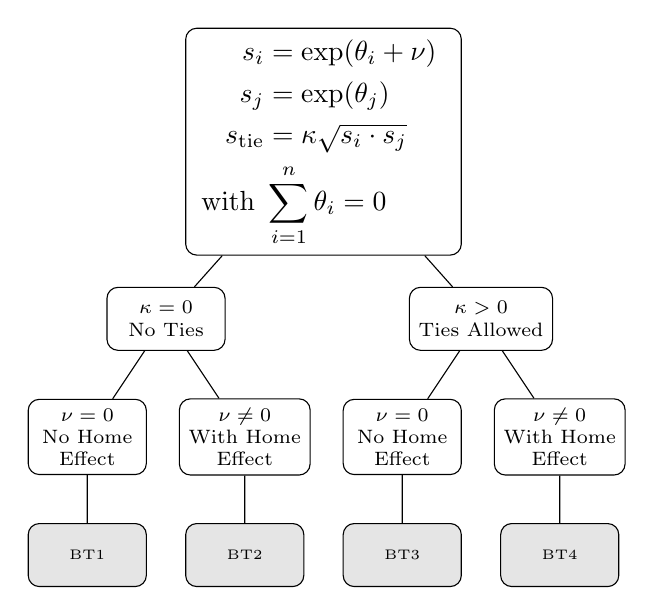
\begin{tikzpicture}[
            level 1/.style = {sibling distance = 4cm, level distance = 2.25cm},
            level 2/.style = {sibling distance = 2cm, level distance = 1.5cm},
            every node/.style = {
                draw,
                rectangle,
                rounded corners,
                align=center,
                minimum width = 1.5cm,
                minimum height = 0.8cm,
                font = \scriptsize
            },
            root/.style = {
                minimum width = 3.5cm,
                minimum height = 1.5cm,
                font = \normalsize
            },
            leaf/.style = {
                fill = gray!20,
                font = \tiny
            }
        ]
            \node[root] {
                $\begin{aligned}
                    s_i &= \exp(\theta_i + \nu) \\
                    s_j &= \exp(\theta_j) \\
                    s_{\text{tie}} &= \kappa \sqrt{s_i \cdot s_j} \\
                    \text{with } &\sum_{i=1}^{n} \theta_i = 0
                \end{aligned}$
            }
                child {
                    node {
                        $\kappa = 0$ \\
                        No Ties
                    }
                    child {
                        node {
                            $\nu = 0$ \\
                            No Home \\
                            Effect
                        }
                        child {
                            node[leaf] {BT1}
                        }
                    }
                    child {
                        node {
                            $\nu \neq 0$ \\
                            With Home \\
                            Effect
                        }
                        child {
                            node[leaf] {BT2}
                        }
                    }
                }
                child {
                    node {
                        $\kappa > 0$ \\
                        Ties Allowed
                    }
                    child {
                        node {
                            $\nu = 0$ \\
                            No Home \\
                            Effect
                        }
                        child {
                            node[leaf] {BT3}
                        }
                    }
                    child {
                        node {
                            $\nu \neq 0$ \\
                            With Home \\
                            Effect
                        }
                        child {
                            node[leaf] {BT4}
                        }
                    }
                };
        \end{tikzpicture}
    \end{center}
\end{frame}

\begin{frame}{Poisson -- Model Taxonomy}
    \begin{center}
    \scalebox{0.7}{%
    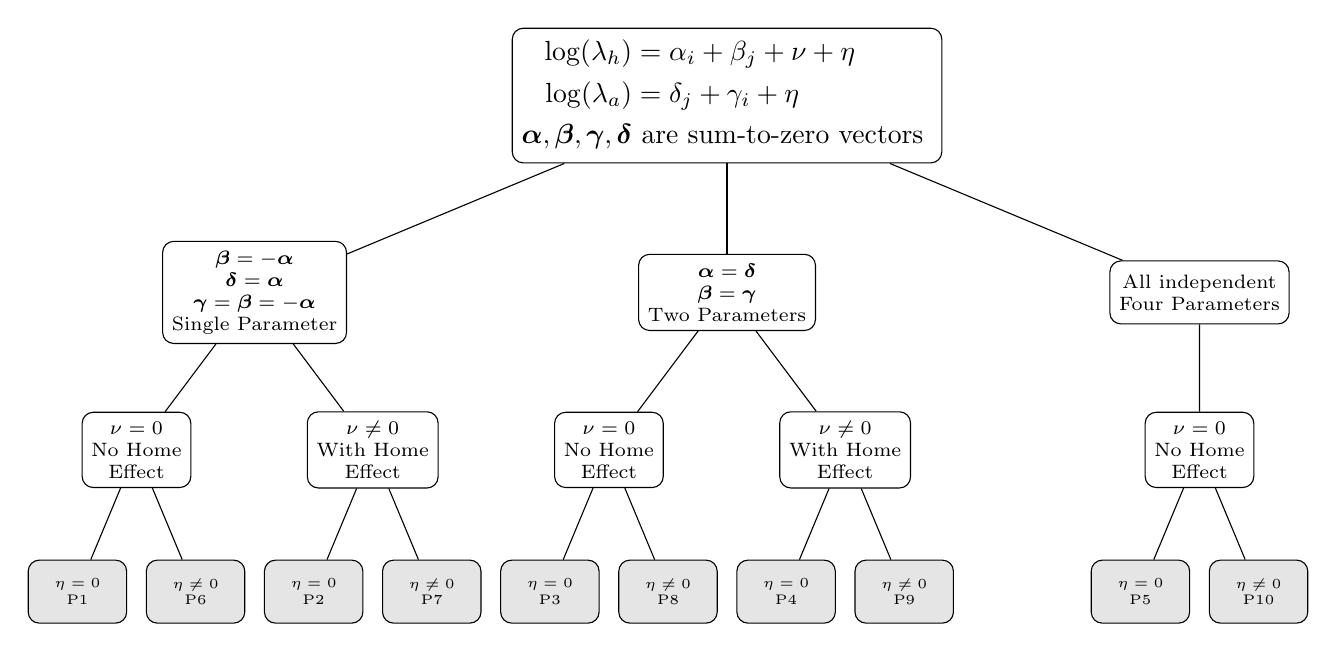
\begin{tikzpicture}[
        level 1/.style = {sibling distance = 6cm, level distance = 2.5cm},
        level 2/.style = {sibling distance = 3cm, level distance = 2cm},
        level 3/.style = {sibling distance = 1.5cm, level distance = 1.8cm},
        every node/.style = {
            draw,
            rectangle,
            rounded corners,
            align=center,
            minimum width = 1.25cm,
            minimum height = 0.8cm,
            font = \scriptsize
        },
        root/.style = {
            minimum width = 3.5cm,
            minimum height = 1.5cm,
            font = \normalsize
        },
        leaf/.style = {
            fill = gray!20,
            font = \tiny
        }
    ]
        \node[root] {
            $\begin{aligned}
                \log(\lambda_{h}) &= \alpha_i + \beta_j + \nu + \eta \\
                \log(\lambda_{a}) &= \delta_j + \gamma_i + \eta \\
                \boldsymbol{\alpha}, \boldsymbol{\beta}, \boldsymbol{\gamma}, \boldsymbol{\delta} &\text{ are sum-to-zero vectors}
            \end{aligned}$
        }
            child {
                node {
                    $\boldsymbol{\beta} = -\boldsymbol{\alpha}$ \\
                    $\boldsymbol{\delta} = \boldsymbol{\alpha}$ \\
                    $\boldsymbol{\gamma} = \boldsymbol{\beta} = -\boldsymbol{\alpha}$ \\
                    Single Parameter
                }
                child {
                    node {
                        $\nu = 0$ \\
                        No Home \\
                        Effect
                    }
                    child {
                        node[leaf] {
                            $\eta = 0$ \\ P1
                        }
                    }
                    child {
                        node[leaf] {
                            $\eta \neq 0$ \\ P6
                        }
                    }
                }
                child {
                    node {
                        $\nu \neq 0$ \\
                        With Home \\
                        Effect
                    }
                    child {
                        node[leaf] {
                            $\eta = 0$ \\ P2
                        }
                    }
                    child {
                        node[leaf] {
                            $\eta \neq 0$ \\ P7
                        }
                    }
                }
            }
            child {
                node {
                    $\boldsymbol{\alpha} = \boldsymbol{\delta}$ \\
                    $\boldsymbol{\beta} = \boldsymbol{\gamma}$ \\
                    Two Parameters
                }
                child {
                    node {
                        $\nu = 0$ \\
                        No Home \\
                        Effect
                    }
                    child {
                        node[leaf] {
                            $\eta = 0$ \\ P3
                        }
                    }
                    child {
                        node[leaf] {
                            $\eta \neq 0$ \\ P8
                        }
                    }
                }
                child {
                    node {
                        $\nu \neq 0$ \\
                        With Home \\
                        Effect
                    }
                    child {
                        node[leaf] {
                            $\eta = 0$ \\ P4
                        }
                    }
                    child {
                        node[leaf] {
                            $\eta \neq 0$ \\ P9
                        }
                    }
                }
            }
            child {
                node {
                    All independent \\
                    Four Parameters
                }
                child {
                    node {
                        $\nu = 0$ \\
                        No Home \\
                        Effect
                    }
                    child {
                        node[leaf] {
                            $\eta = 0$ \\ P5
                        }
                    }
                    child {
                        node[leaf] {
                            $\eta \neq 0$ \\ P10
                        }
                    }
                }
            };
    \end{tikzpicture}%
    }
    \end{center}
\end{frame}

\begin{frame}{Player-Level Extension}
    We replace the team skill with aggregated player skills:
    \begin{equation*}
        s_{\text{team}} = \sum_{p \in \mathcal{P}} \exp(\theta_p) \cdot \frac{m_p}{90}
    \end{equation*}

    \begin{itemize}
        \item $\theta_p$ is the individual log-skill, with $\sum_p \theta_p = 0$;

        \item we use a synthetic player with an estimable parameter $\theta_{\text{synthetic}}$ to model the impact of red cards.
    \end{itemize}
\end{frame}

%===================================================
% 4. SIMULATION-BASED CALIBRATION
%===================================================
\section{Simulation-Based Calibration}

\begin{frame}[fragile]{SBC -- Workflow}
    \begin{center}
    \scalebox{1.1}{%
    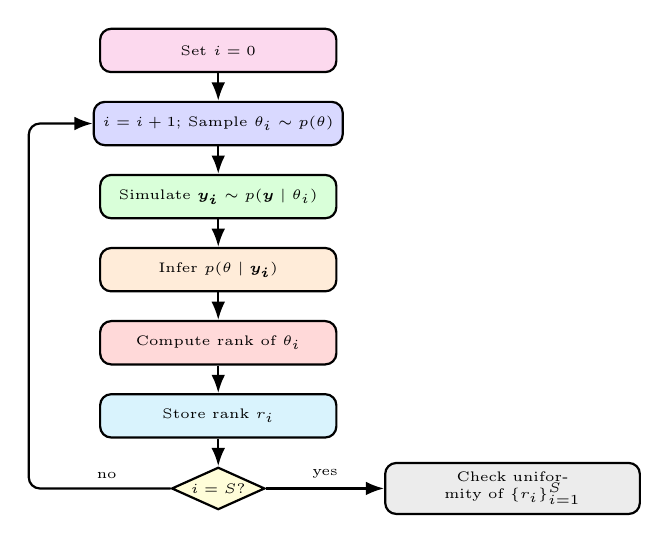
\begin{tikzpicture}[
        node distance=0.35cm,
        >=Latex,
        thick,
        process/.style={draw, rounded corners, minimum width=3cm, minimum height=0.55cm, align=center, font=\tiny, fill=#1!15},
        process/.default=blue,
        decision/.style={diamond, aspect=2.2, draw, align=center, inner sep=1pt, fill=yellow!15, font=\tiny}
    ]
        \node[process=magenta] (start) {Set $i = 0$};
        \node[process=blue, below=of start] (sample) {$i = i + 1$; Sample $\theta_i \sim p(\theta)$};
        \node[process=green, below=of sample] (simulate) {Simulate $\boldsymbol{y_i} \sim p(\boldsymbol{y} \mid \theta_i)$};
        \node[process=orange, below=of simulate] (infer) {Infer $p(\theta \mid \boldsymbol{y_i})$};
        \node[process=red, below=of infer] (rank) {Compute rank of $\theta_i$};
        \node[process=cyan, below=of rank] (store) {Store rank $r_i$};
        \node[decision, below=of store] (check) {$i = S$?};
        \node[process=gray, right=1.5cm of check, text width=3cm] (aggregate) {Check uniformity of $\{r_i\}_{i=1}^S$};

        \draw[->] (start) -- (sample);
        \draw[->] (sample) -- (simulate);
        \draw[->] (simulate) -- (infer);
        \draw[->] (infer) -- (rank);
        \draw[->] (rank) -- (store);
        \draw[->] (store) -- (check);
        \draw[->] (check.east) -- node[above, pos=0.5]{\tiny yes} (aggregate.west);
        \draw[->, rounded corners] (check.west) -- node[above, pos=0.45]{\tiny no} +(-1.8,0) |- (sample.west);
    \end{tikzpicture}%
    }
    \end{center}
\end{frame}

\begin{frame}{SBC -- Diagnostics}
    \begin{columns}[T]
    \begin{column}{0.4\textwidth}
        \begin{figure}
            \centering
            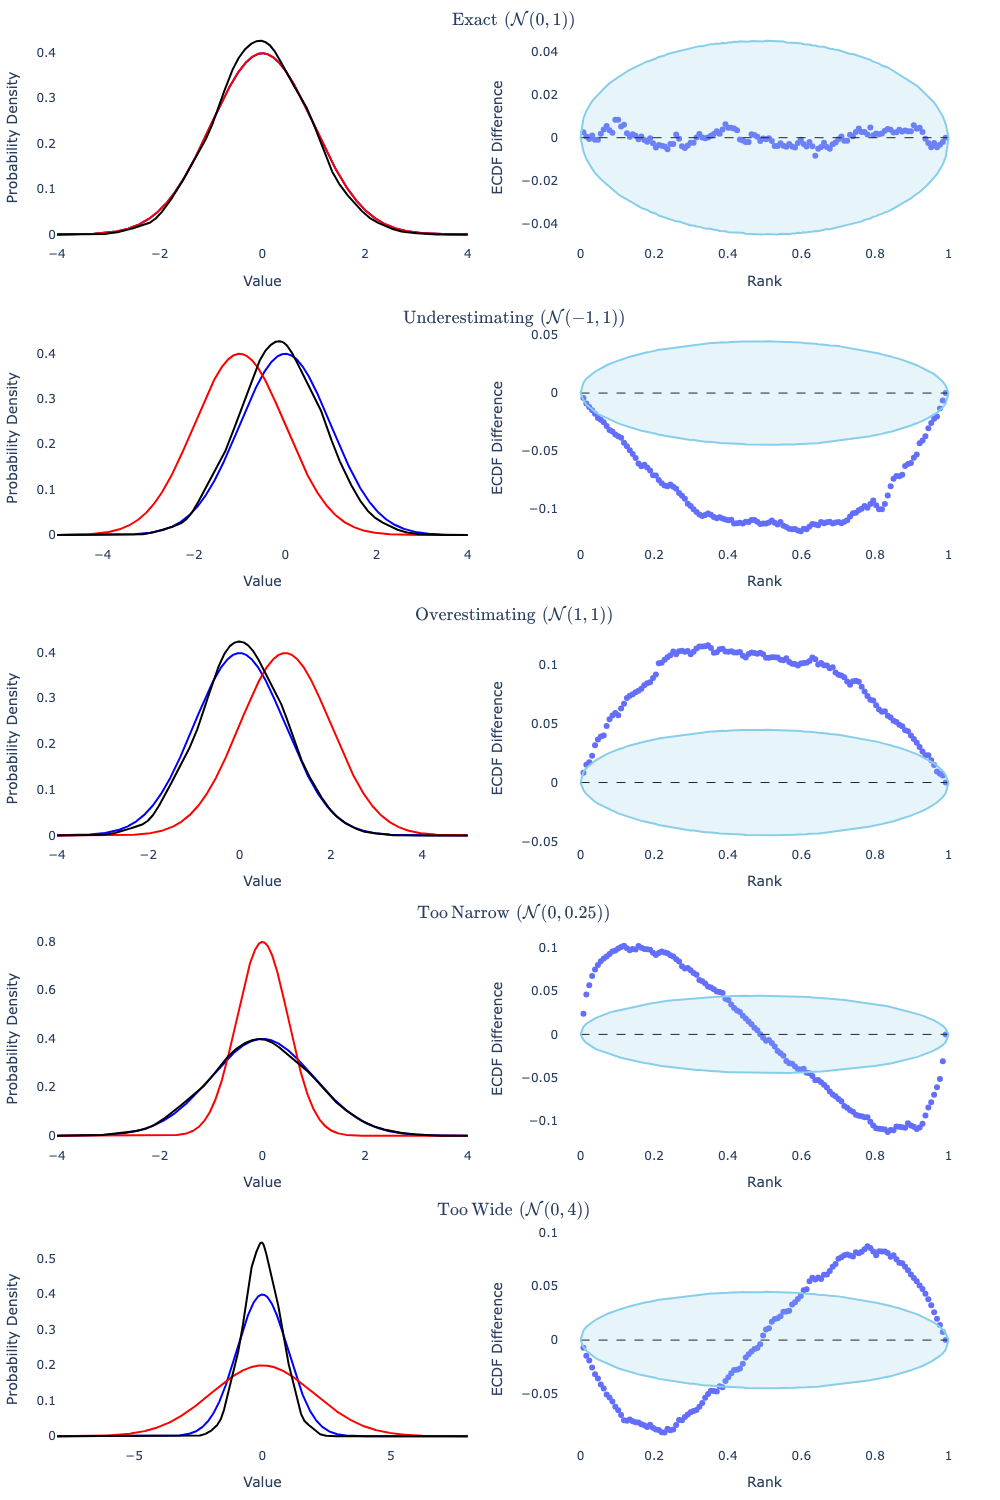
\includegraphics[width=\textwidth]{figures/sbc_visualization.png}
        \end{figure}
    \end{column}
    \begin{column}{0.48\textwidth}
        \vspace{0.8cm}
        \begin{itemize}
            \item \textbf{Flag}: $\geq 1$ ECDF point outside the envelope for a parameter;

            \item \textbf{Points Out}: total violations across all rank values in that model;

            \item Expected flagging rate under correct calibration: $\approx 5\%$.
        \end{itemize}
    \end{column}
    \end{columns}
\end{frame}

%===================================================
% 5. RESULTS
%===================================================
\section{Results}

\begin{frame}{Scoring Rules}
    Let $\mathbf{z}_t$ be the outcome and $\mathbf{p}_t$ the predicted probabilities.

    \setlistsep{1.2ex}{1ex}{1ex}
    \begin{itemize}
        \item \textbf{Brier Score}:
        \[\text{BS} = \frac{1}{n} \sum_{t=1}^{n} \sum_{j} (z_{j,t} - p_{j,t})^2\]

        \item \textbf{Log Score}:
        \[\text{LS} = -\frac{1}{n} \sum_{t=1}^{n} \sum_{j} z_{j,t} \log(p_{j,t})\]

        \item \textbf{Ranked Probability Score}:
        \[\text{RPS} = \frac{1}{2n} \sum_{t=1}^{n} \sum_{k=1}^{2} \!\left( \sum_{j=1}^{k} (z_{j,t} - p_{j,t}) \right)^{\!2}\]
    \end{itemize}
\end{frame}

\begin{frame}{Club-Level Model Comparison}
    \begin{table}[h]
        \centering
        \scriptsize
        \begin{tabular}{lcccc}
            \toprule
            Model & BS & RPS & LS & Description \\
            \midrule
            Naive 1 & 0.6667 & 0.2359 & 1.0986 & Equal probabilities \\
            Naive 2 & 0.6373 & 0.2243 & 1.0570 & Historical proportions \\
            \midrule
            BT3     & 0.6494 & 0.2293 & 1.0768 & Bradley-Terry with ties \\
            BT4     & 0.6508 & 0.2296 & 1.0800 & BT3 + home effect \\
            \midrule
            P1  & 0.6497 & 0.2287 & 1.0741 & Simple Poisson \\
            P2  & 0.6256 & 0.2180 & 1.0402 & P1 + home effect \\
            P3  & 0.6558 & 0.2324 & 1.0860 & Attack/defence \\
            P4  & 0.6356 & 0.2230 & 1.0550 & P3 + home effect \\
            P5  & 0.6834 & 0.2460 & 1.1255 & Home/away split \\
            P6  & 0.6495 & 0.2286 & 1.0738 & P1 + common effect \\
            \textbf{P7}  & \textbf{0.6237} & \textbf{0.2172} & \textbf{1.0378} & \textbf{P2 + common effect} \\
            P8  & 0.6548 & 0.2318 & 1.0840 & P3 + common effect \\
            P9  & 0.6334 & 0.2218 & 1.0526 & P4 + common effect \\
            P10 & 0.6835 & 0.2460 & 1.1263 & P5 + common effect \\
            \bottomrule
        \end{tabular}
        \caption*{
            Predictive performance on \textit{Brasileirão} 2020--2025. Lower values are better; best model is in bold.
        }
    \end{table}
\end{frame}

\begin{frame}{Match-Level Parameters by Season (P7)}
    \begin{table}[h]
        \centering
        \footnotesize
        \begin{tabular}{lcccc}
            \toprule
            Season & $\nu$ (95\% CI) & $\exp(\nu)$ & $\eta$ (95\% CI) & $\exp(\eta)$ \\
            \midrule
            2020 & 0.273 (0.15, 0.40) & 1.31 & 0.031 ($-$0.07, 0.13) & 1.03 \\
            2021 & 0.296 (0.16, 0.43) & 1.34 & $-$0.096 ($-$0.20, 0.00) & 0.91 \\
            2022 & 0.365 (0.23, 0.50) & 1.44 & $-$0.075 ($-$0.18, 0.04) & 0.93 \\
            2023 & 0.281 (0.14, 0.40) & 1.32 & 0.028 ($-$0.07, 0.13) & 1.03 \\
            2024 & 0.310 (0.19, 0.44) & 1.36 & $-$0.003 ($-$0.11, 0.09) & 1.00 \\
            2025 & 0.425 (0.29, 0.55) & 1.53 & $-$0.062 ($-$0.16, 0.04) & 0.94 \\
            \bottomrule
        \end{tabular}
        \caption*{
            Summary of the posterior distributions of the home effect parameter ($\nu$) and the common effect parameter ($\eta$) across seasons.
        }
    \end{table}
\end{frame}

\begin{frame}{Team Strengths -- 2025}
    \begin{figure}
        \centering
        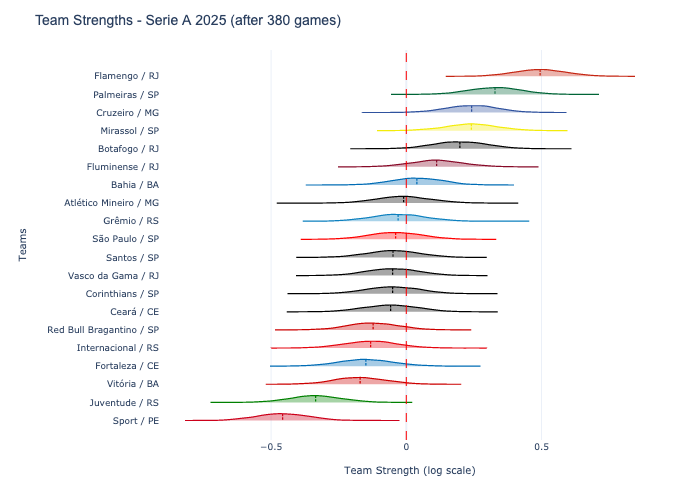
\includegraphics[width=0.8\textwidth]{figures/2025_team_strengths_violin.png}
        \caption*{
            Posterior distributions of the team strength parameter (log scale) for each club, ordered by posterior median strength.
        }
    \end{figure}
\end{frame}

\begin{frame}{Player Rankings (2020--2025)}
    \tiny
    \setlength{\tabcolsep}{2pt}
    \renewcommand{\arraystretch}{0.9}
    \setlength{\columnsep}{3pt}

    \begin{columns}[T,totalwidth=\textwidth]
        \begin{column}{0.495\textwidth}
            \centering
            \begin{tabular}{@{}rlcccc@{}}
                \toprule
                \multicolumn{6}{c}{\textbf{Top 20}}\\
                \midrule
                \# & Player & Club & Med & 95\% CI & WGD \\
                \midrule
                1  & Weverton     & PAL & 0.132 & [$-$0.07, 0.33] & 153.5 \\
                2  & Arrascaeta   & FLA & 0.093 & [$-$0.10, 0.30] & 106.7 \\
                3  & F. Bruno     & FLA & 0.083 & [$-$0.12, 0.28] & 94.2  \\
                4  & G. Gómez     & PAL & 0.083 & [$-$0.12, 0.29] & 105.5 \\
                5  & Murilo       & PAL & 0.082 & [$-$0.12, 0.28] & 96.4  \\
                6  & J. Piquerez  & PAL & 0.079 & [$-$0.12, 0.28] & 99.9  \\
                7  & Marcos Rocha & PAL & 0.076 & [$-$0.12, 0.27] & 91.1  \\
                8  & R. Veiga     & PAL & 0.076 & [$-$0.13, 0.28] & 93.0  \\
                9  & Léo Pereira  & FLA & 0.067 & [$-$0.13, 0.27] & 84.0  \\
                10 & Zé Rafael    & PAL & 0.064 & [$-$0.14, 0.26] & 82.3  \\
                11 & A. Rossi     & FLA & 0.063 & [$-$0.14, 0.26] & 74.0  \\
                12 & Éverson      & CAM & 0.060 & [$-$0.14, 0.26] & 72.0  \\
                13 & Renê         & INT & 0.058 & [$-$0.14, 0.26] & 61.0  \\
                14 & Rony         & PAL & 0.056 & [$-$0.14, 0.25] & 73.1  \\
                15 & Léo Ortiz    & RBB & 0.055 & [$-$0.15, 0.25] & 64.7  \\
                16 & Pedro        & FLA & 0.052 & [$-$0.15, 0.25] & 65.9  \\
                17 & B. Henrique  & FLA & 0.052 & [$-$0.15, 0.25] & 64.7  \\
                18 & Ayrton Lucas & FLA & 0.052 & [$-$0.15, 0.25] & 61.6  \\
                19 & Gerson       & FLA & 0.050 & [$-$0.15, 0.25] & 63.5  \\
                20 & Cuesta       & INT & 0.050 & [$-$0.15, 0.25] & 55.3  \\
                \bottomrule
            \end{tabular}
        \end{column}

        \begin{column}{0.495\textwidth}
            \centering
            \begin{tabular}{@{}rlcccc@{}}
                \toprule
                \multicolumn{6}{c}{\textbf{Bottom 20}}\\
                \midrule
                \# & Player & Club & Med & 95\% CI & WGD \\
                \midrule
                1956 & Victor Luis    & BOT & $-$0.026 & [$-$0.22, 0.17] & $-$32.7 \\
                1957 & Lucas          & AME & $-$0.026 & [$-$0.22, 0.17] & $-$34.7 \\
                1958 & Rodrigo Alves  & JUV & $-$0.026 & [$-$0.22, 0.16] & $-$34.4 \\
                1959 & Pedro Raul     & CEA & $-$0.026 & [$-$0.22, 0.16] & $-$37.9 \\
                1960 & Victor Hugo    & BAH & $-$0.027 & [$-$0.22, 0.16] & $-$36.8 \\
                1961 & Shaylon        & ATG & $-$0.028 & [$-$0.22, 0.17] & $-$36.6 \\
                1962 & R. Thyere      & SPO & $-$0.028 & [$-$0.22, 0.17] & $-$37.2 \\
                1963 & Lucas Halter   & GOI & $-$0.029 & [$-$0.22, 0.16] & $-$39.1 \\
                1964 & C. Rivera      & SPO & $-$0.029 & [$-$0.22, 0.16] & $-$39.5 \\
                1965 & Gilberto       & BAH & $-$0.030 & [$-$0.22, 0.16] & $-$38.8 \\
                1966 & Matheus        & CUI & $-$0.030 & [$-$0.22, 0.16] & $-$37.9 \\
                1967 & G. Baralhas    & ATG & $-$0.031 & [$-$0.23, 0.16] & $-$44.6 \\
                1968 & Éder           & ATG & $-$0.034 & [$-$0.22, 0.16] & $-$46.0 \\
                1969 & Tadeu          & GOI & $-$0.035 & [$-$0.22, 0.15] & $-$48.0 \\
                1970 & Matheusinho    & SPO & $-$0.036 & [$-$0.23, 0.16] & $-$41.3 \\
                1971 & I. Pitta       & CUI & $-$0.037 & [$-$0.23, 0.15] & $-$48.8 \\
                1972 & Kevin          & AVA & $-$0.037 & [$-$0.23, 0.15] & $-$47.6 \\
                1973 & Lucas Lima     & SPO & $-$0.044 & [$-$0.24, 0.15] & $-$54.0 \\
                1974 & Jadson         & JUV & $-$0.050 & [$-$0.24, 0.14] & $-$66.4 \\
                1975 & G. Vasconcelos & COR & $-$0.051 & [$-$0.24, 0.14] & $-$71.4 \\
                \bottomrule
            \end{tabular}
        \end{column}
    \end{columns}
\end{frame}

%===================================================
% 6. CONCLUSION
%===================================================
\section{Conclusion}

\begin{frame}{Conclusion}
    \begin{itemize}
        \item Model P7 (single skill + home + common effect) performs best;
        
        \item Split attack/defence by home/away does not improve performance;
        
        \item The common effect parameter is not statistically significant;
        
        \item Home effect is significant: home team expected goals between 1.31 and 1.53 times when playing away;
        
        \item Player-level rankings reflect team context ($r \approx 0.99$ with WGD).
    \end{itemize}
\end{frame}

\begin{frame}{Future Work}
    \begin{itemize}
        \item Player-specific event data for finer attribution;

        \item Dynamic models: team/player abilities evolving over time;

        \item Contextual covariates: fatigue, travel, match importance;

        \item All code is available at \url{https://github.com/BrazilianFootball}.
    \end{itemize}
\end{frame}

\begin{frame}{}
    \centering
    \vspace{2cm}
    {\Large Thank you!}
\end{frame}

\end{document}
